\apendice{Documentación técnica de programación}

\section{Introducción}
En este apartado se va a explicar todo lo relacionado con el código desarrollado durante el proyecto. Desde la estructura de directorios y archivos que componen el proyecto, hasta los pasos necesarios para  compilar, instalar y ejecutar el proyecto de diferentes formas.
\section{Estructura de directorios}
Todo el código relacionado con el proyecto se encuentra en un repositorio público en
GitHub\footnote{\href{http://github.com/VictorDeMarco/IoT_data_gestion}{http://github.com/VictorDeMarco/IoT\_data\_gestion}}. 

A continuación, se va a mostrar la estructura de directorios y archivos que se pueden encontrar en el repositorio del proyecto:


\begin{itemize}
    \item \textbf{examples}: directorio que contiene archivos csv de ejemplo para probar las distintas funcionalidades del proyecto.
   \item \textbf{docs}: directorio que contiene los archivos referentes a la documentación del proyecto:
   \begin{itemize}
       \item \textbf{anexo}: directorio que contiene los archivos referentes a los anexos del proyecto.
       \item \textbf{memoria}: Directorio que contiene los archivos referentes a la memoria del proyecto.
       \item \textbf{videos}: Directorio que contiene Readme.md con los enlaces a los videos explicativos.
   \end{itemize}
    \item \textbf{src}: directorio que contiene los archivos referentes al código fuente del proyecto:
    \begin{itemize}
       \item \textbf{csv}: directorio donde se almacenan todos los ficheros csv utilizados por el proyecto,en este directorio también se crean las carpetas personales de cada usuario que utiliza la aplicación dashboard.
       \item \textbf{dashboard\_visualizer}: directorio principal de la aplicación de visualización y gestión de archivos csv.
       \item \textbf{webhook\_receptor}: directorio principal de la aplicación de recepción, análisis y almacenamiento de datos  enviados por sensores IoT.
   \end{itemize}
   
   \item \textbf{docker}: directorio que contiene los archivos necesarios para ejecutar el proyecto en un contenedor docker.

   \item \textbf{.gitignore}: archivo de configuración de Git que contiene los elementos a omitir en el control de versiones.

   \item \textbf{README.md}: archivo de presentación del proyecto donde se resume en qué consiste el proyecto y diversos puntos importantes del mismo.
   
\end{itemize}

Dentro del directorio \textbf{docker} se encuentran los siguientes archivos:

\begin{itemize}
    \item \textbf{docker-compose.yml}: archivo de configuración que permite configurar y ejecutar múltiples contenedores Docker como un solo proyecto.
    \item \textbf{Dockerfile}: archivo necesario para desplegar el proyecto en un contenedor Docker.
    \item \textbf{requirements.txt}: archivo que contiene las bibliotecas necesarias para ejecutar correctamente el proyecto.
\end{itemize}

Dentro del directorio \textbf{src/dashboard\_visualizer} se encuentran los siguientes archivos y directorios:

\begin{itemize}
    \item \textbf{instance}: directorio donde se guarda la instancia de la base de datos encargada de gestionar los usuarios de la aplicación.
    \item \textbf{routes}: directorio que contiene los archivos de código con las funcionalidades de la aplicación.
    \item \textbf{templates}: directorio que contiene todas las plantillas de las distintas vistas de la aplicación.
    \item \textbf{utils}: directorio que contiene utilidades secundarias para el funcionamiento de la aplicación.
    \item \textbf{dashboard\_flask.py}: archivo principal de la aplicación encargado de iniciar la misma.
\end{itemize}

Dentro del directorio \textbf{src/webhook\_receptor} se encuentran los siguientes archivos y directorios:

\begin{itemize}
    \item \textbf{rules}: directorio donde se guarda un pequeño scrypt encargado de la generación de reglas de asociación.
    \item \textbf{webhook\_flask.py}: archivo principal de la aplicación encargado de iniciar la misma y de todas sus funcionalidades, como recibir y analizar datos.
\end{itemize}

Dentro del directorio \textbf{src/webhook\_receptor/rules} se encuentran los siguientes archivos y directorios:
\begin{itemize}
    \item \textbf{rules.py}: archivo principal con el scrypt encargado de generar las reglas.
    \item \textbf{csv\_rules}: directorio donde se guarda el archivo csv con solo datos reales del sensor IoT, utilizado para generar las reglas de asociación.
\end{itemize}



\section{Manual del programador}
En este apartado se explica como crear el entorno de desarrollo necesario para desplegar el proyecto.

Lo primero seria obtener el código completo del proyecto , ya sea descargándolo directamente de GitHub\footnote{\href{http://github.com/VictorDeMarco/IoT_data_gestion}{http://github.com/VictorDeMarco/IoT\_data\_gestion}} o clonando el repositorio\footnote{git clone https://github.com/VictorDeMarco/IoT\_data\_gestion.git} .

Una vez se dispone del código completo del proyecto es necesario instalar las siguientes herramientas:

\begin{itemize}
    \item Python >=3.10-2 o <=3.11
    \item Docker desktop
    \item Git
    \item Navegador web 
    \item IDE (Intellij)
    \item Aceso a compilador LaTeX
\end{itemize}


\section{Compilación, instalación y ejecución del proyecto}
El proyecto se puede ejecutar de dos formas, las cuales se van a explicar a continuación.

\label{ejec_local}
\subsection{Ejecución en local}
Primero se va a explicar el método de ejecución en local:

Suponiendo que se han cumplido todos los pasos mencionados
anteriormente lo primero que debemos hacer es instalar las dependencias necesarias para el proyecto, para ello ejecutaremos el siguiente comando desde la carpeta principal del proyecto \textbf{IoT\_data\_gestion}:

\begin{verbatim}
    pip install -r docker\requirements.txt
\end{verbatim}

El siguiente paso es ejecutar el scrypt principal para iniciar cualquiera de las dos aplicaciones web que componen el proyecto. 

Para la aplicación webhook:

\begin{verbatim}
    python -m src.webhook_receptor.webhook_flask
\end{verbatim}

Para la aplicación dashboard: 

\begin{verbatim}
    python -m src.dashboard_visualizer.dashboard_flask
\end{verbatim}

Para ejecutar el scrypt que genera las reglas de asociación utilizadas durante el análisis de los paquetes de datos recibidos los pasos son:

Comenzando en la carpeta principal del proyecto nos movemos hasta donde se encuentra el scrypt:
\begin{verbatim}
    cd .\src\webhook_receptor\rules\
\end{verbatim}

Y ejecutamos el siguiente comando una vez estamos en la carpeta correspondiente:
\begin{verbatim}
    python rules.py
\end{verbatim}

Este script solo puede ser ejecutado de manera local y mostrará en la terminal el resultado de su ejecución.

\label{ejec_docker}
\subsection{Ejecución en Docker}

Por último se va a explicar el método de ejecución en Docker:

Lo primero es instalar docker desktop en tu dispositivo, puedes hacerlo desde este enlace:

\href{https://www.docker.com/products/docker-desktop/}{https://www.docker.com/products/docker-desktop/}

Asegúrate de descargar el instalador correspondiente a tu sistema operativo.

Ejecutar el instalador y seguir los pasos guiados y una vez finalizada la instalación, reiniciar el sistema si es necesario.

Una vez instalado docker desktop, ejecuta la aplicación.

Luego desde la carpeta principal del proyecto \textbf{IoT\_data\_gestion} ejecuta el siguiente comando para componer el contenedor docker con todos los servicios y dependencias necesarias:

\begin{verbatim}
    docker-compose -f docker\docker-compose.yml up
\end{verbatim}

Una vez ejecutado el comando en tu docker desktop deberia verse algo similar a esto:

\begin{figure}
    \centering
    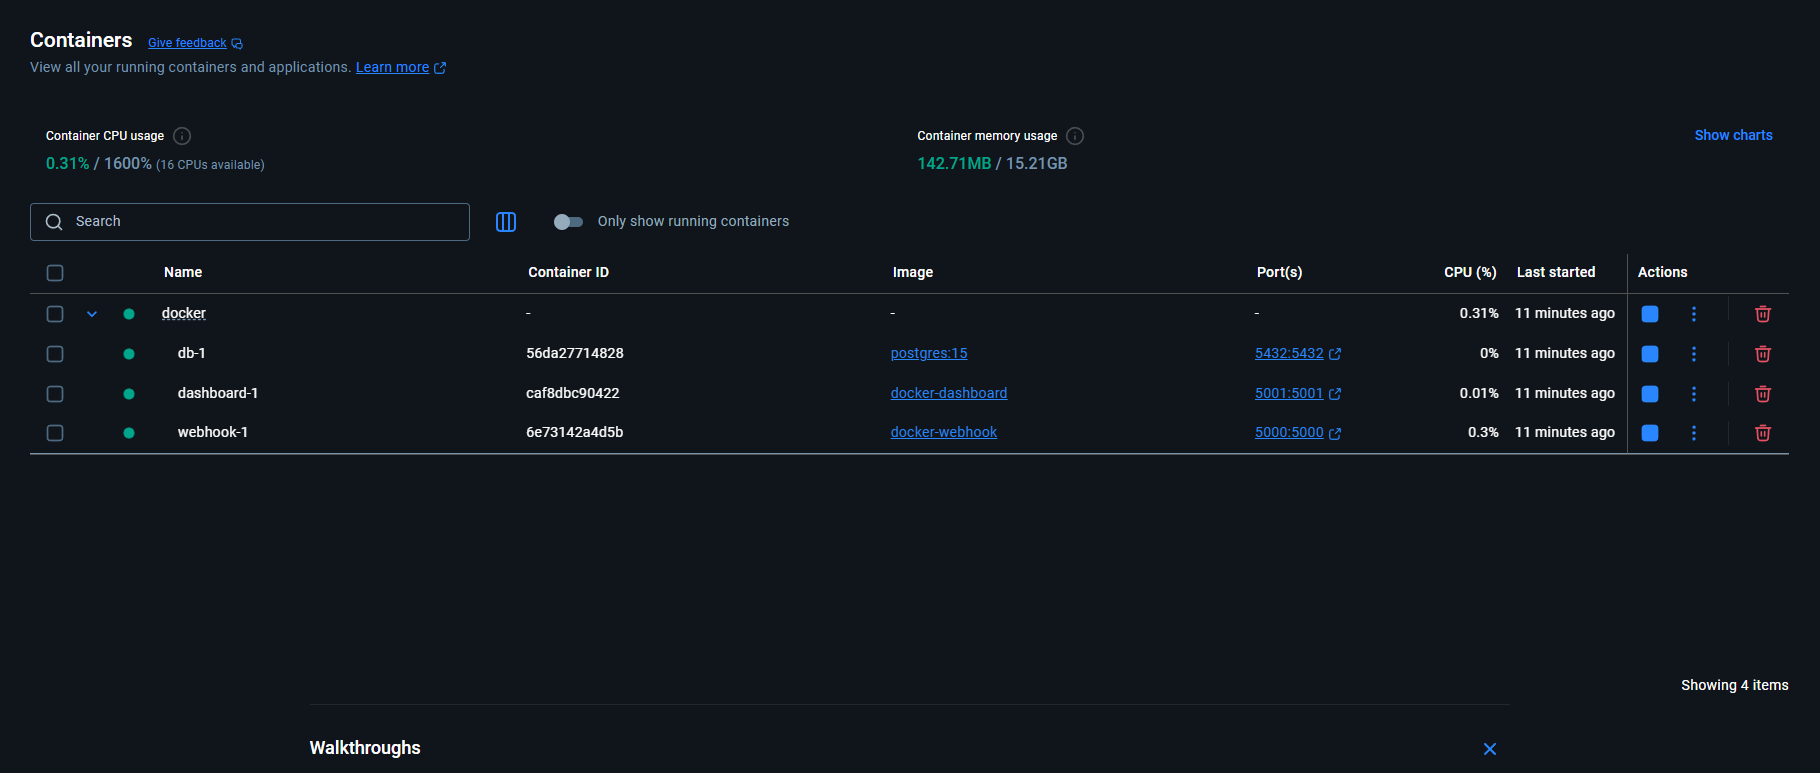
\includegraphics[width=1\textwidth]{contenedor_docker} 
    \caption{Imagen de la correcta construcción del contenedor docker}
\end{figure}

Si todo ha funcionado ambas aplicaciones se deben haber ejecutado correctamente y puedes acceder a la aplicación con interfaz diseñada para el usuario desde un navegador usando el siguiente enlace:

\href{http://localhost:5001/}{http://localhost:50001/}


\section{Pruebas del sistema}
Una vez finalizado el proyecto, se realizaron distintas pruebas para asegurar que el sistema funcione correctamente.

En la aplicación \textbf{webhook\_flask} se probó que el sistema fuera capaz de soportar recibir peticiones erróneas o mal formuladas, notificándolo por la terminal.

En la aplicación \textbf{dashboard\_flask} se realizaron diversas pruebas para asegurar la integridad del proyecto, desde evitar que el usuario intentara dejar en blanco algún campo de los diversos formularios de la aplicación hasta controlar que el usuario no pueda borrar el archivo base del dataset, evitando así problemas severos en la estructura del proyecto.

También se probo que el usuario no pudiera cargar archivos no soportados por la aplicación evitando así un desajuste en el funcionamiento de la aplicación.




